Find the Fourier Series for the tent function defined by:

\[
f(x) = \begin{cases}
    1 + x, & x \in (-1, 0) \\
    1 - x, & x \in (0, 1)
\end{cases}, \; f(x) = f(x + 2)
\]

\begin{solution}\ \\\\
    We first solve for $a_0$ with the observation that $L = 1$:
    \begin{flalign*}
        a_0 &= \frac{1}{2L} \int_{-L}^{L}{f(x)\; dx}  &\\
            &= \frac{1}{2} \int_{-1}^{0}{1 + x \; dx} 
             + \frac{1}{2} \int_{0}^{1}{1 - x \; dx} &\\
            &= \frac{1}{2}
    \end{flalign*}
    
    Next, we find the Fourier cosine coefficients:
    \begin{flalign*}
        a_n &= \frac{1}{L} \int_{-L}^{L}{f(x) \cos{\left( \frac{n \pi x}{L}\right)} \; dx} &\\
            &= \int_{-1}^{0}{(1 + x) \cos{\left(n \pi x\right)}\; dx} 
             + \int_{0}^{1}{(1 - x) \cos{\left(n \pi x\right)}\; dx} &\\
            &= \frac{1 - \cos{(\pi n)}}{(\pi n)^2} + \frac{1 - \cos{(\pi n)}}{(\pi n)^2} &\\
            &= \begin{cases}
                \frac{4}{(n \pi)^2} & \text{if $n$ is odd} \\
                0 & \text{if $n$ is even}
            \end{cases}
    \end{flalign*}
    
    Lastly, we solve for the Fourier sine coefficients, which we expect \textit{a priori} to be 0 since our tent 
    function $f(x)$ is even:
    \begin{flalign*}
        b_n &= \frac{1}{L} \int_{-L}^{L}{f(x) \sin{\left( \frac{n \pi x}{L}\right)} \; dx}  &\\
            &= \int_{-1}^{0}{(1 + x) \sin{\left(n \pi x\right)}\; dx} 
             + \int_{0}^{1}{(1 - x) \sin{\left(n \pi x\right)}\; dx} &\\
            &= -\frac{1}{\pi n} + \frac{1}{\pi n} &\\
            &= 0.
    \end{flalign*}
   
    \pagebreak
    The Fourier series representation of $f(x)$ is therefore given by (reindexing $a_n$ for conciseness): 

    \begin{align*}
    f(x) &\sim a_0 + \sum\limits_{n=1}^{\infty}{a_n \cos{\left(\frac{n \pi x}{L}\right)} + b_n \sin{\left(\frac{n \pi x}{L}\right)}} \\
         &= \frac{1}{2} + \sum\limits_{n=1}^{\infty}{\frac{4}{\pi^2 (2n - 1)^2} \cos{[(2n - 1) \pi x]}}
    \end{align*}

    Lastly, we show the 1-term and 5-term Fourier series approximations to $f(x)$:

    \begin{figure*}[h]
        \centering
        \begin{subfigure}[b]{0.475\textwidth}
            \centering
            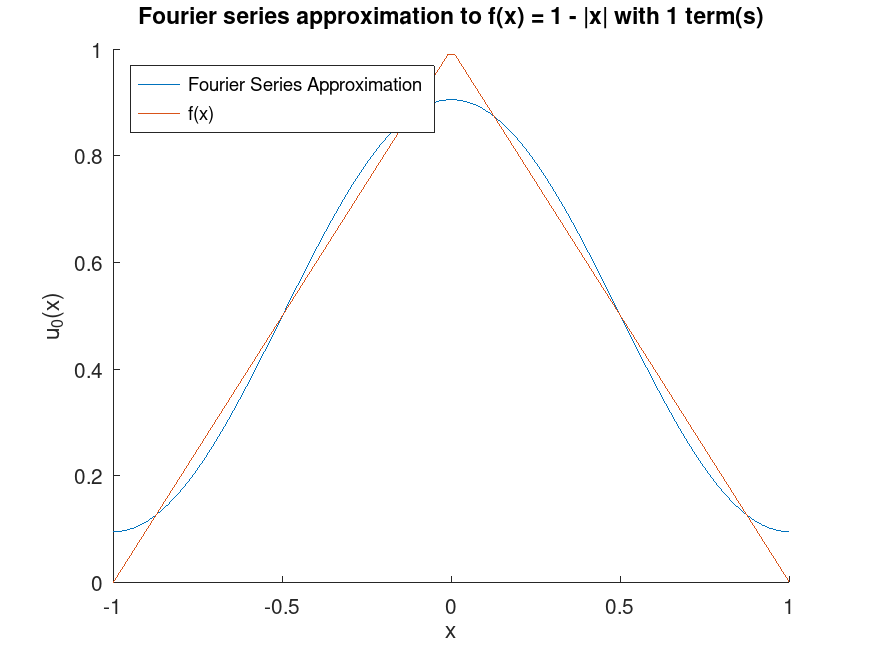
\includegraphics[width=\textwidth]{problem1_fourier_series_solution_1_term.png}
            \label{fig:problem1_5terms}
        \end{subfigure}
        \hfill
        \begin{subfigure}[b]{0.475\textwidth}
            \centering
            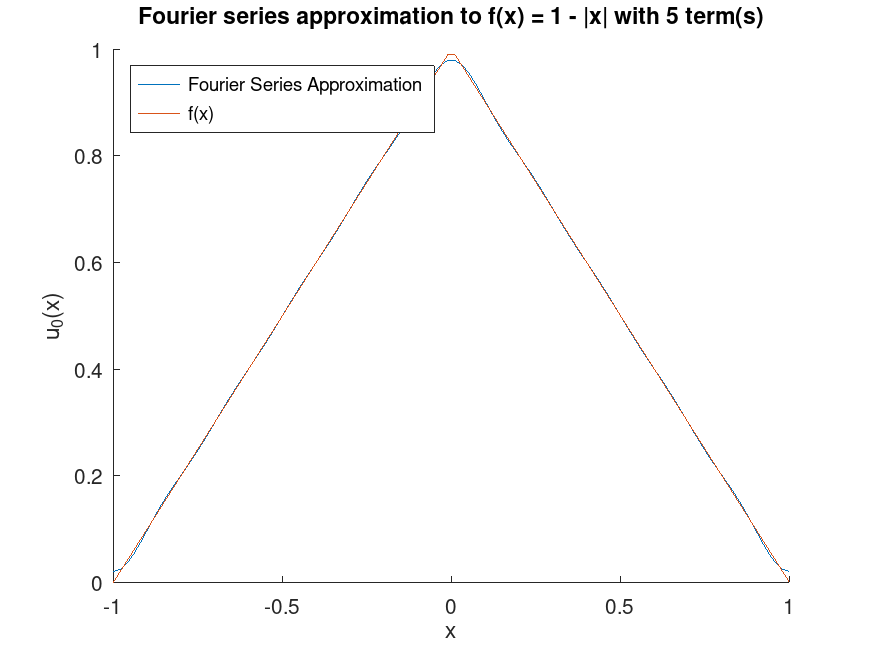
\includegraphics[width=\textwidth]{problem1_fourier_series_solution_5_term.png}
            \label{fig:problem1_50terms}
        \end{subfigure}
        \caption[Fourier Series solution]
        {\small Fourier Series approximations to $f(x) = 1 - |x|$} 
        \label{fig:fouriersoln}
    \end{figure*}
\end{solution}

